\begin{frame}[ctb]
\frametitle{Sensitivity Analysis with the Clay Generic Disposal System Model}

Recall : Abstraction process uses results from more detailed models to improve 
speed and accuracy of analytical models. In this case, sensitivity analyses were 
conducted using the Used Fuel Disposition Campaign's Clay Generic Disposal System 
Model \cite{huff_key_2012} in order to inform the analytic models just discussed.

\begin{table}[ht!]
\centering
\footnotesize{
\begin{tabular}{|l|l|l|r|r|}
\multicolumn{5}{c}{\textbf{Simulation Cases}}\\
\hline
\textbf{Case} & \textbf{Parameter} & \textbf{Units} & \textbf{Min. Value} & \textbf{Max. Value}\\
\hline
I     & $D_{eff}$    & $[m^2\cdot s^{-1}]$       & $10^{-8}$    &  $10^{-5}$ \\
      & Inventory              & [MTHM]         & $10^{-4}$    &  $10^1$ \\
\hline
II    & $V_{adv, y}$ & $[m \cdot yr^{-1}]$       & $6.31\times10^{-8}$  &  $6.31\times10^{-4}$ \\
      & $D_{eff}$    & $[m^2\cdot s^{-1}]$       & $10^{-8}$    &  $10^{-5}$ \\
\hline
III   & $S_i$        & $[mol\cdot m^{-3}]$       & $(1\times10^{-9})\langle S_i\rangle $    &  $(5\times10^{10})\langle S_i\rangle $ \\
\hline
IV    & $K_{d,i}$    & $[m^3\cdot kg^{-1}]$       & $(1\times10^{-9})\langle K_{d,i}\rangle $    &  $(5\times10^{10})\langle K_{d,i}\rangle $ \\
\hline
V     & $R_{WFDeg.}$           & $[yr^{-1}]$       & $10^{-9}$    &  $10^{-2}$ \\
      & Inventory              & [MTHM]         & $10^{-4}$    &  $10^1$ \\
\hline 
VI    & $t_{WPFail}$        & $[yr]$         & $10^3$    &  $10^7$ \\
      & $D_{eff}$           & $[m^2\cdot s^{-1}]$       & $10^{-8}$    &  $10^{-5}$ \\
\hline
\end{tabular}
\caption{Each dual and single parameter simulation case had 40 simulation 
groups of 100 realizations each.}
\label{tab:Cases}
}
\end{table}



\end{frame}


\begin{frame}[ctb]
\frametitle{Solubility Sensitivity}
\begin{figure}[ht]
  \centering
  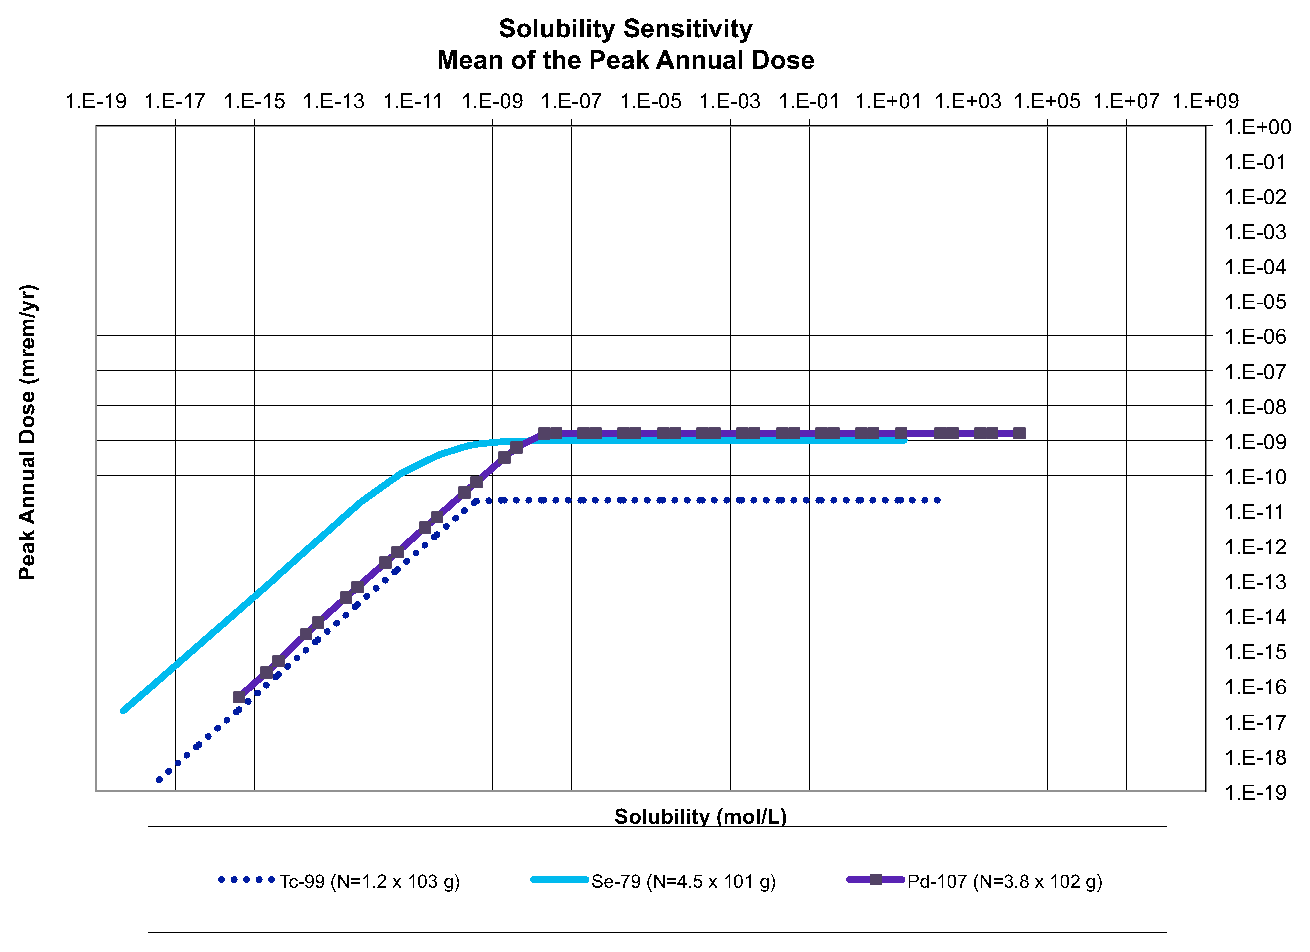
\includegraphics[height=60mm]{cyder/images/Solubility_Summary.eps}
  \caption{Generated with the Used Fuel Disposition Campaign's Generic Disposal 
  System Model for Clay, this graph demonstrates solubility limit sensitivity. 
  The peak annual dose due to an inventory, $N$, of each isotope.}
  \label{fig:SolSum}
\end{figure}
\end{frame}

\begin{frame}[ctb]
\frametitle{Retardation Sensitivity}
\begin{figure}[ht]
  \centering
  \includegraphics[height=60mm]{cyder/images/Partitioning_Summary.eps}
  \caption{Generated with the Used Fuel Disposition Campaign's Generic Disposal 
  System Model for Clay, this graph demonstrates $K_d$ sensitivity. 
  The peak annual dose due to an inventory, $N$, of each isotope.}
  \label{fig:KdSum}
\end{figure}
\end{frame}


